\documentclass[8pt,a4paper]{beamer}
\usepackage[utf8]{inputenc}
\usepackage[output-decimal-marker={,}]{siunitx}
\usepackage[compat=1.1.0]{tikz-feynman}
\author{Adriano Del Vincio}
\title{Beam normal single spin asymmetry measurement at MAMI}


\begin{document}

\frame{\titlepage}

\begin{frame}{Beam-time 29/11/2022 - 5/12/2022}
\framesubtitle{Beam normal single spin asymmetry}
During the last beam-time, several mesurements were performed at Mainz Mikrotron MAMI. The last data acquisition campaign had the following goals:

\begin{itemize}
\item Test the new data acquisition system, developed for the new setup with a low rate signals ($\simeq \SI{1}{\mega \hertz} $). 
\item Measure the trasverse asymmetry $A_{n}$ of $^{12}C$.
\item Measure the expected rates on $^{208}Pb$ target, in anticipation of the future mesurement of $A_{n}$ for lead. 
\item Long term goal: acquire more knowledge on the systematic effects that the transverse asymmetry has on the measurement of the Parity-violating asymmetry.
\end{itemize}

\end{frame}

\begin{frame}{A first look the physics of the problem}

Before moving on to the experimental details, we identify the kinematics of the experiment. For the beam normal single spin asymmetry, the electrons are polarized in the normal plane identified by the $\frac{\vec{k'} \wedge \vec{k}}{ |\vec{k}| |\vec{k'}|}$ 

\begin{figure}[hbtp]
\centering
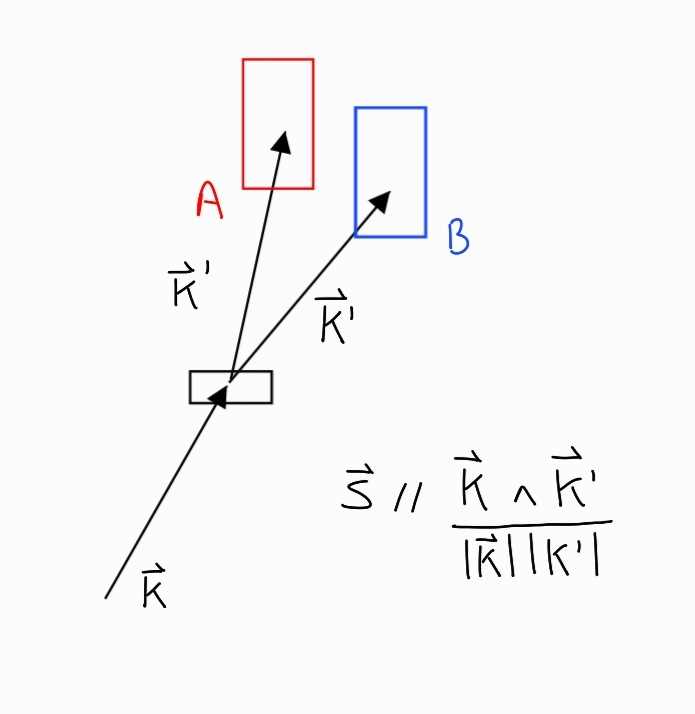
\includegraphics[width = 0.35\textwidth]{figures/SmartSelect_20221204_171028_Samsung Notes.jpg}
\hspace{2cm}
\includegraphics[width = 0.30\textwidth]{figures/IMG_20221124_144946.jpg} 
\caption{(very) schematic figure of the experiment on the left, Spektrometers B (blue) and A on right, view is from the beam dump}
\end{figure}
The position of the two dectector is fixed at $\simeq 23 ^{\circ}$, that correspond to a $Q^{2} = \SI{0.04} {\giga \electronvolt}$

\end{frame}

\begin{frame}{Structure of the event}

The trasverse asymmetry is defined as the ratio between the sum and the difference of the elastic cross section for the two different polarized electrons: 

\begin{equation*}
A_{transverse} = \dfrac{\sigma_{\uparrow} -  \sigma_{\downarrow}}{\sigma_{\uparrow} + \sigma_{\downarrow}}
\end{equation*}

straightforward this quantity can be measured with the asymmetry in the counts of a detector. With the following convention, the beam is polarized (using a de bruijn sequence) in one of the two possible configuration of the spin. So an event corresponds to the integration of all particles scattered during 80 ms window. 

\begin{figure}[hbtp]
\centering
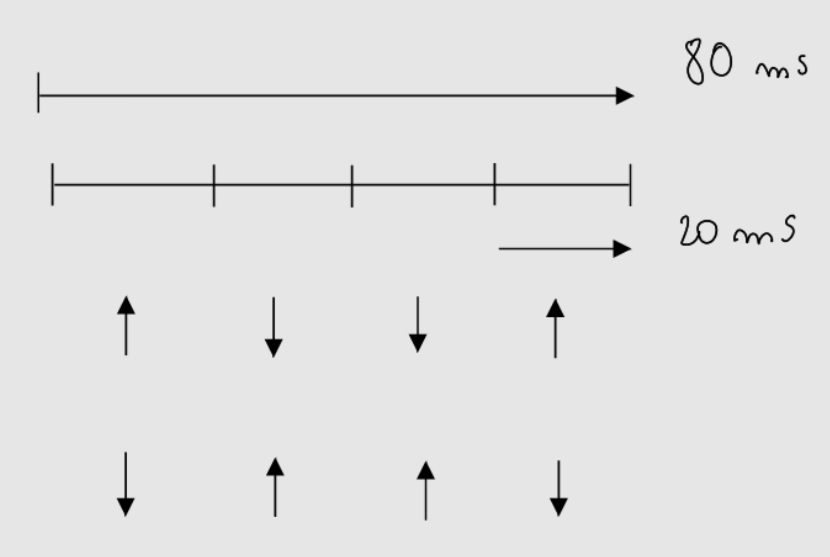
\includegraphics[width = 0.5\textwidth]{figures/EventStructure.jpg}
\caption{Event sequence: all the particle}
\end{figure}


\end{frame}


\begin{frame}{Scattering process}

The following one is the diagram we are interest to calculate,  the one loop correction to the electron-nucleus elastic scattering. This diagram give rise to a non-zero imaginary part of the elastic amplitude, that is related to the transverse asymmetry.

\begin{figure}[hbtp]
\feynmandiagram [scale = 0.8, transform shape][baseline = (h), horizontal = c to f]{
	a [particle=\(e^{-}\)] -- c -- f -- g [particle = \(e^{-}\)],
	c -- [boson, edge label'= \(\gamma\)] d,
	f -- [boson, edge label'= \(\gamma\)] j,
	h [particle = \(C^{12}\)]-- d --  j -- k [particle = \(C^{12}\)] ,
};
\hspace{2cm}
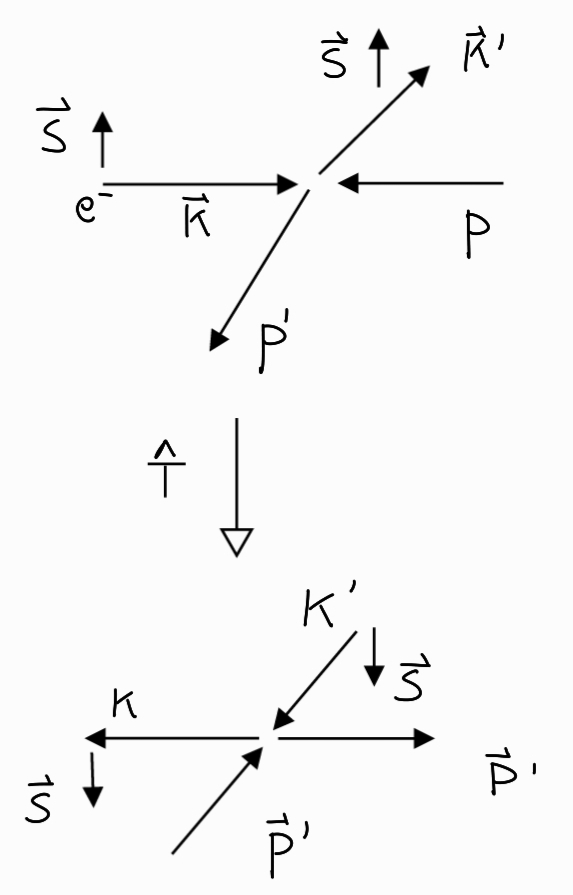
\includegraphics[width = 0.30\textwidth]{figures/time.jpg} 
\end{figure}

If we consider the same scattering process, but after applying $\hat{T}$ operator, the spin of the electron is reversed. This means that the asymmetry is directly correlated to Time-reversal simmetry. 

\end{frame}



\begin{frame}{Scattering Process}

The incident beam is made by $\SI{570}{\mega \electronvolt}$ electrons, that are polarized along the trasverse axes ($\uparrow$ and $\downarrow$). The physical quantity to measure is the asymmetry between the number of scattered electrons, due to the change of the polarity:

\begin{equation}
asym = \frac{N_{+} - N_{-}}{N_{+} + N_{-}} \text{(expected $\sim$ +/- 20 ppm, Q = \SI{0.2}{\giga\electronvolt c^{-1}})}
\end{equation}

It's possible to obtain a final formula for the trasverse Asymmetry, writing the Amplitude of the 1-loop diagram, considering the elastic intermediate state and the inelastic intermediate state (whose contribution is higher):

\begin{equation}
A_{n} \simeq C_{0} \log \frac{Q^{2}}{m^2_e c^2} \frac{F_{Compton} (Q^2)}{F_{ch}(Q^2)}
\end{equation}

It's possible to perform analytical calculation for the inelastic intermediate state, however for the inelastic term, some parametrization are needed.

\end{frame}

\begin{frame}{The Detectors}
The detectors are made by 9 and 3 pmts coupled to a fused-silica material, exploiting the Cherenkov light produced when a particle travel inside the material.

\begin{figure}[hbtp]
\centering
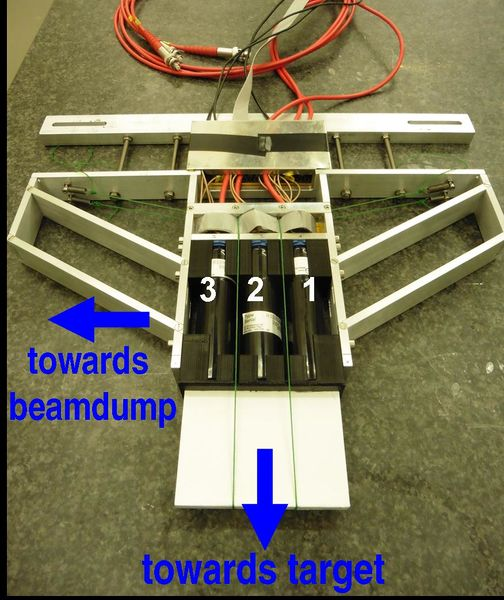
\includegraphics[width = 0.3\textwidth]{figures/504px-Blackfalcon.jpg}
\hspace{2cm}
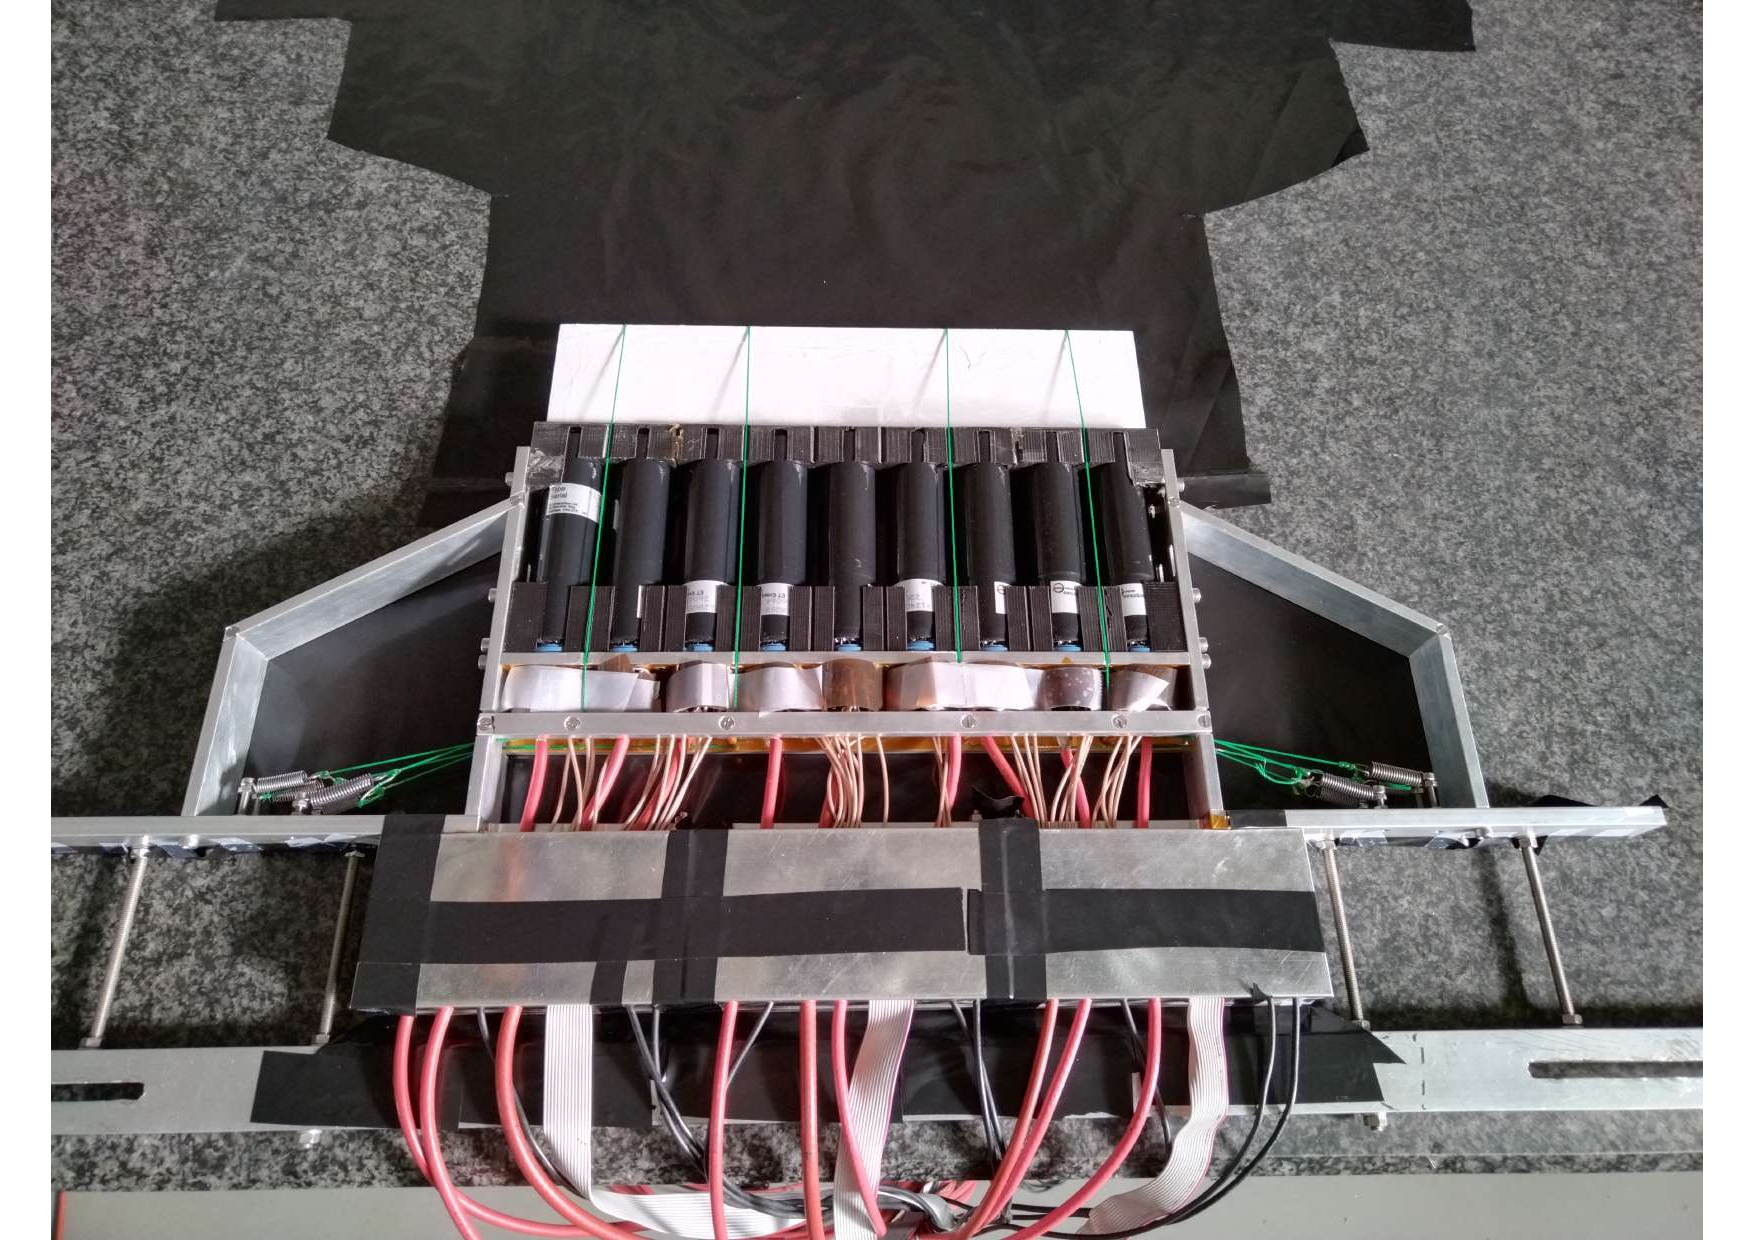
\includegraphics[width = 0.4\textwidth]{figures/IMG_20221110_122246.jpg}
\caption{Detector B on the left, detector A on the right.}
\end{figure}

\end{frame}

\begin{frame}{Read-out}

The pmt signals are read-out by a Nino-board, shown in figure: This device collects the number of pulses directly from the pmts. It’s made by discriminators which compare the input signals (on the left side) to a signal that can be adjusted manually with the pvDaq.py scripts. Three parameters are important for the DAQ and calibration of the pmt: the Voltage supply of the pmts, the threshold (always fixed) and the Attenuation.

\begin{figure}[hbtp]
 
 \centering
 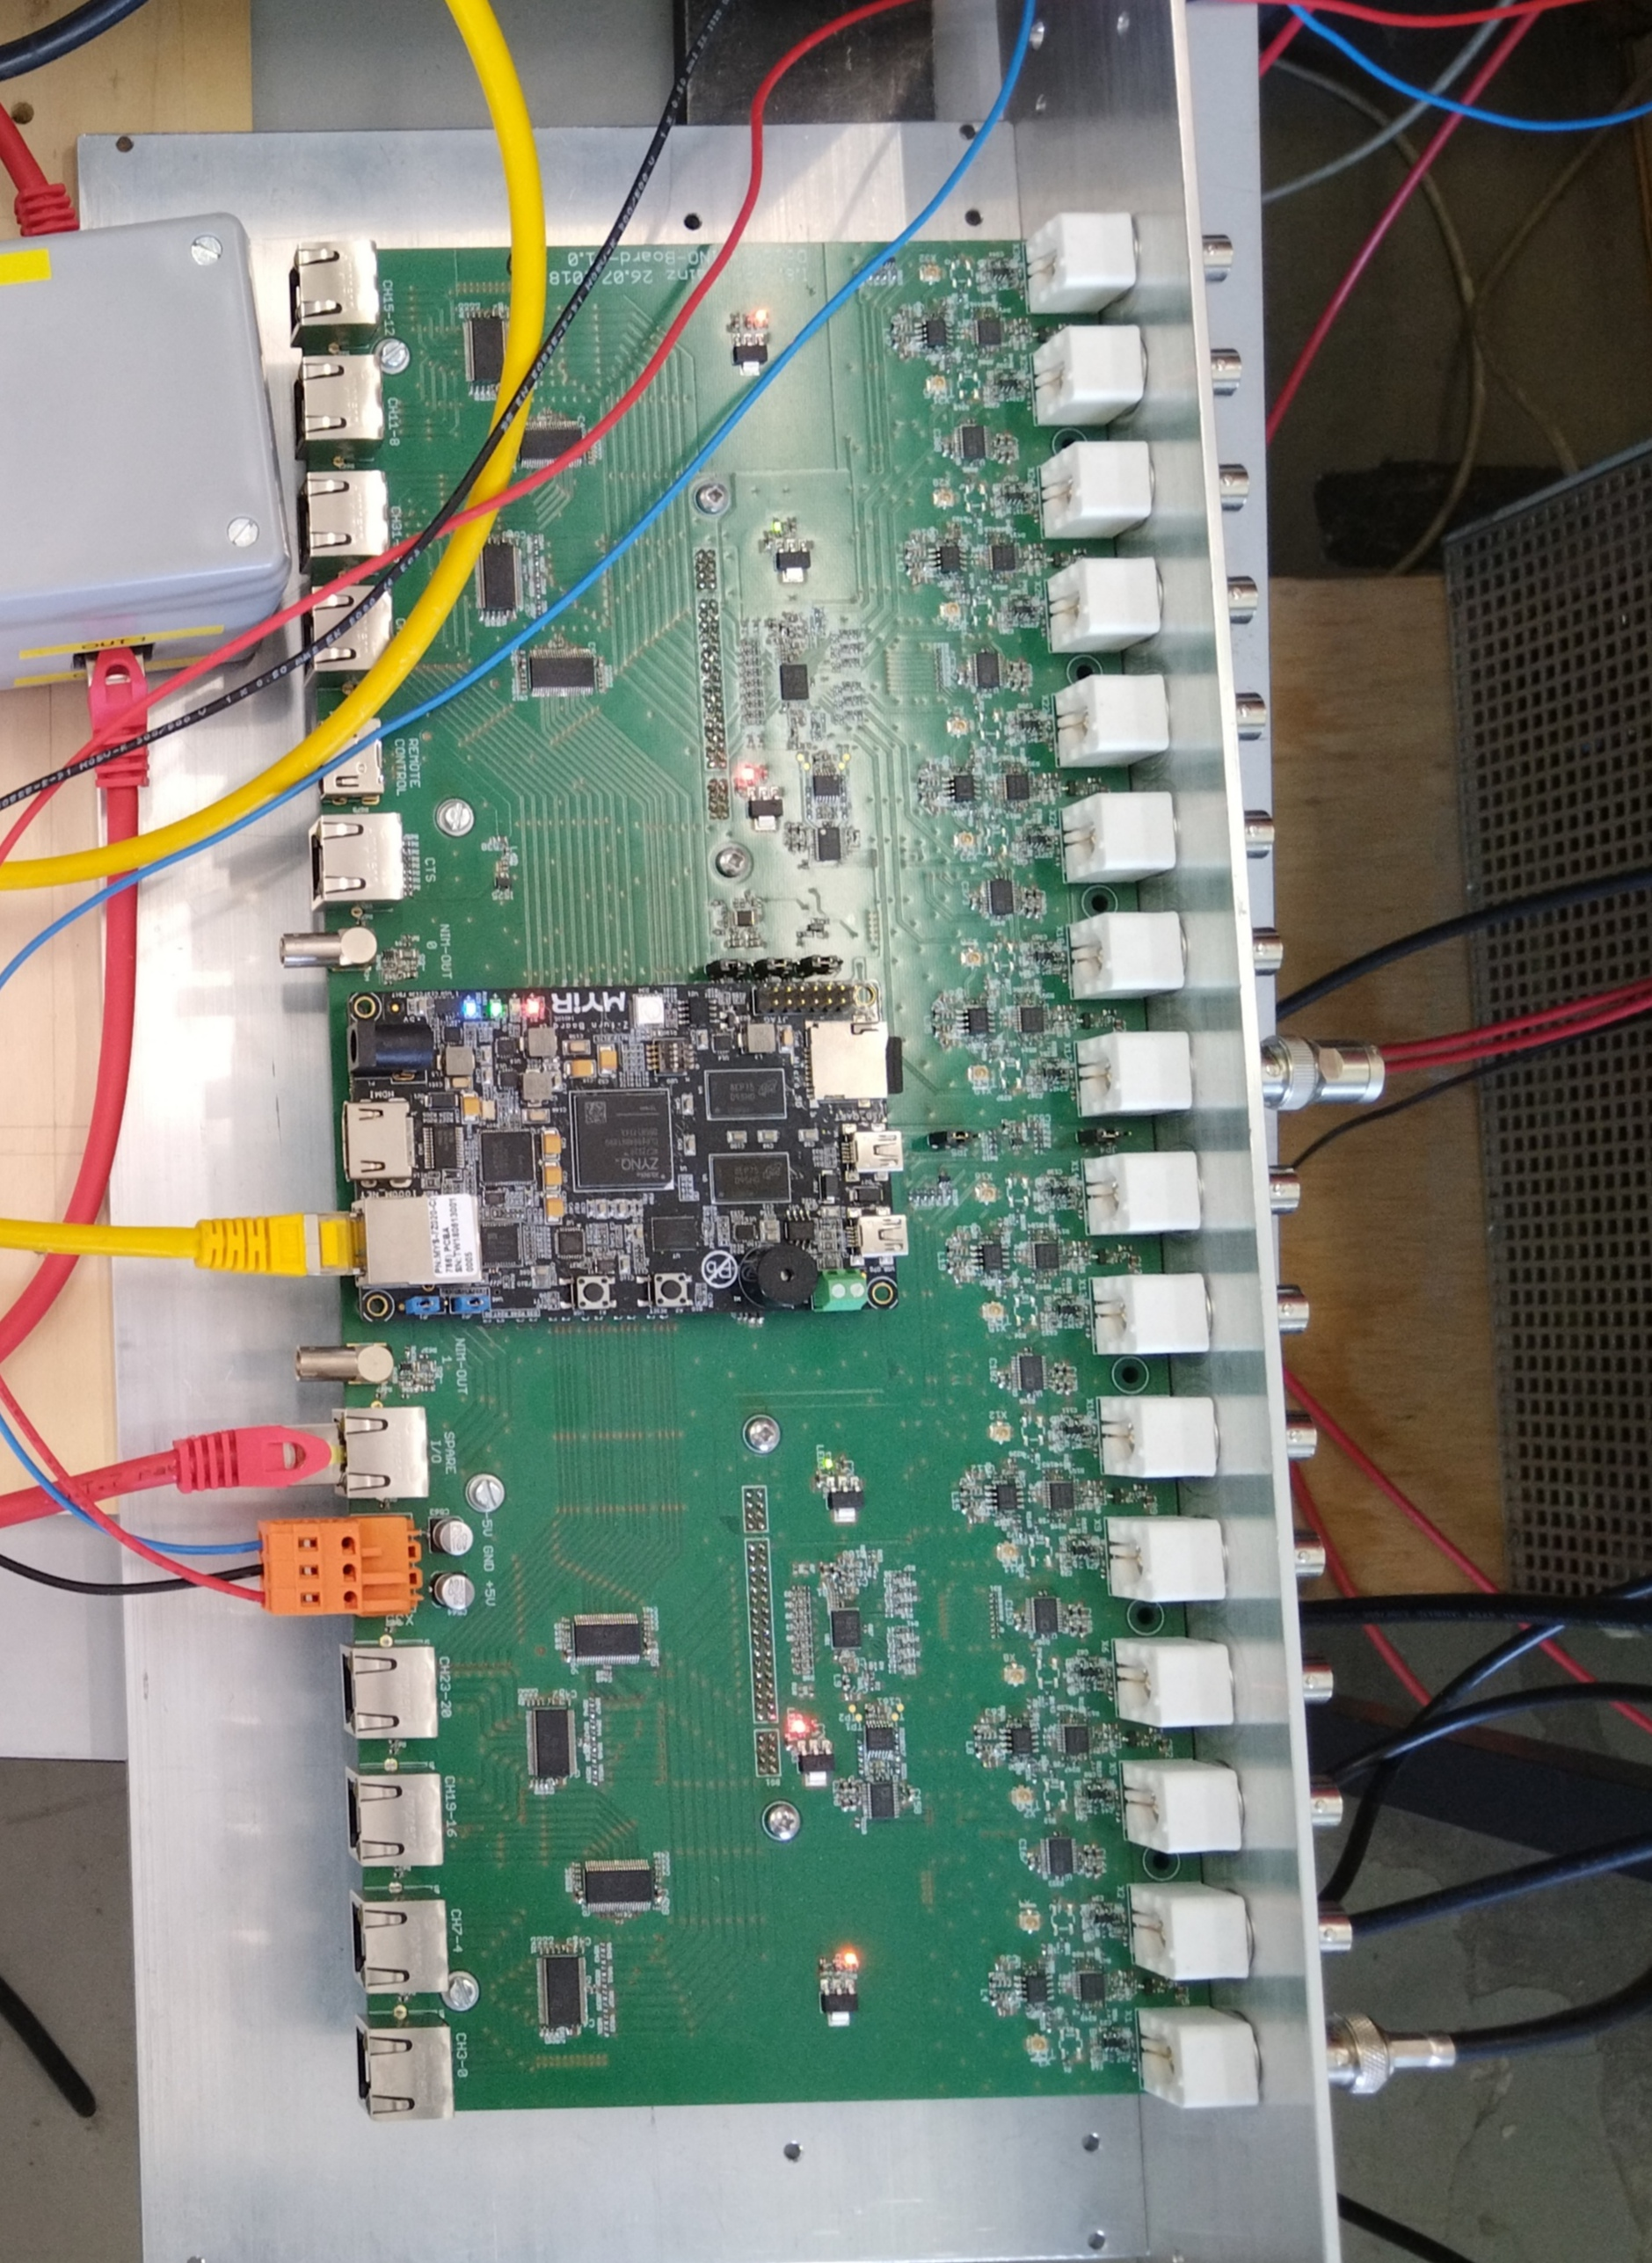
\includegraphics[width = 0.4\textwidth]{figures/NinoBoard.jpg}
 \caption{Nino-Board, on the right the input channels for the signals}
 \end{figure}
  

\end{frame}

\begin{frame}

Here we present a picture of the MasterBoard, the core of the electronics system, which controls and supervises the following functions:

\begin{itemize}
\item it controls the X and Y signals to the Wobbler, to avoid melting the target.
\item it sends the signals to the Source, to change the polarity of the beam ($\simeq 0.79$).
\item it Manages the data from all the beam monitors: X21/25/26, Y21/25/26, I21, I13, ENMO.

\end{itemize}


\begin{figure}
\centering
\includegraphics[width = 0.5\textwidth]{figures/MasterBoard.jpg}
\end{figure}
 
\end{frame}


\begin{frame}{The Detectors}
The detectors are placed inside the two spektrometers, which were used only to align the two detectors to the elastic scattering line (changing the magnetic field).

\begin{figure}[hbtp]
\centering
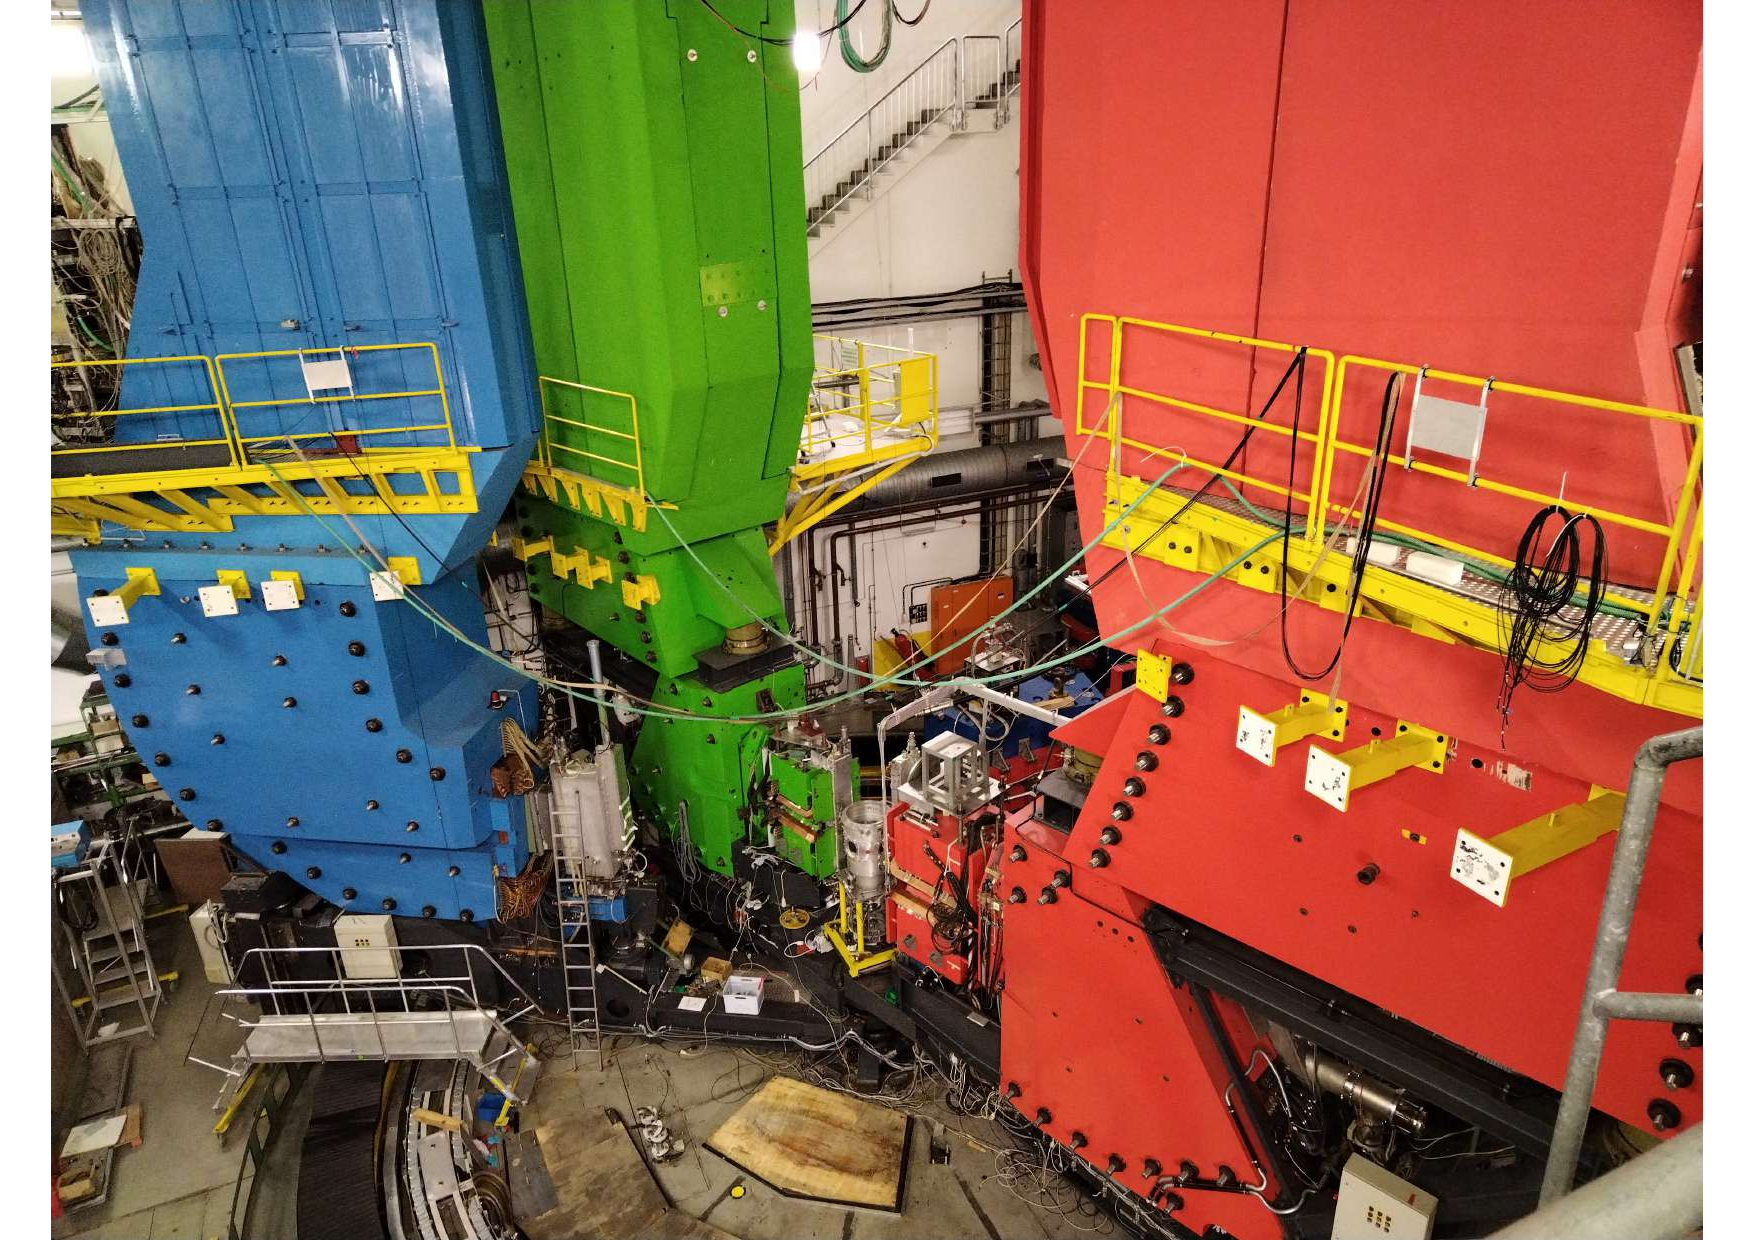
\includegraphics[width = 0.5\textwidth]{figures/twoSpektrometer.jpg}
\hspace{1cm}
\includegraphics[width = 0.3\textwidth]{figures/InsideDetector.jpg} 
\caption{Spektrometers B and A on the left, view of the inside with the detector A in position.}
\end{figure}


\end{frame}

\begin{frame}{Vfc I21 calibration}
\begin{figure}[hbtp]
\centering
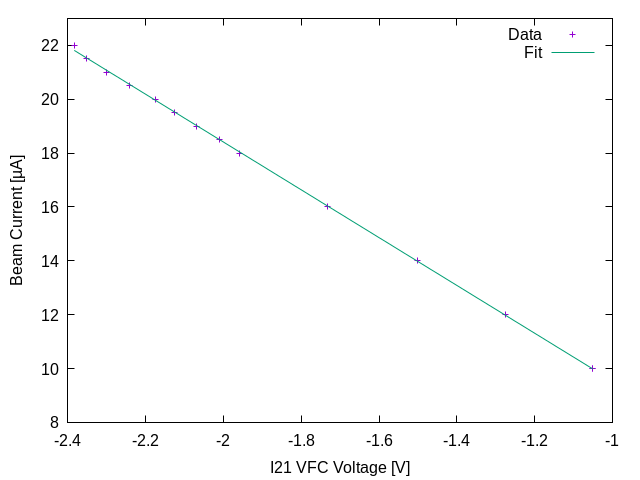
\includegraphics[width = 0.7\textwidth]{figures/Calib_I21_from_Pb_runs.png}
\caption{ Calibration of the VFC I21 monitor, for me measurement of the beam current.}
\end{figure}

\end{frame}

\begin{frame}{Calibration of the pmt}

\begin{figure}[hbtp]
\caption{pmt Count spekA, the threshold was selected at the edge of the knee for each pmt.}
\centering
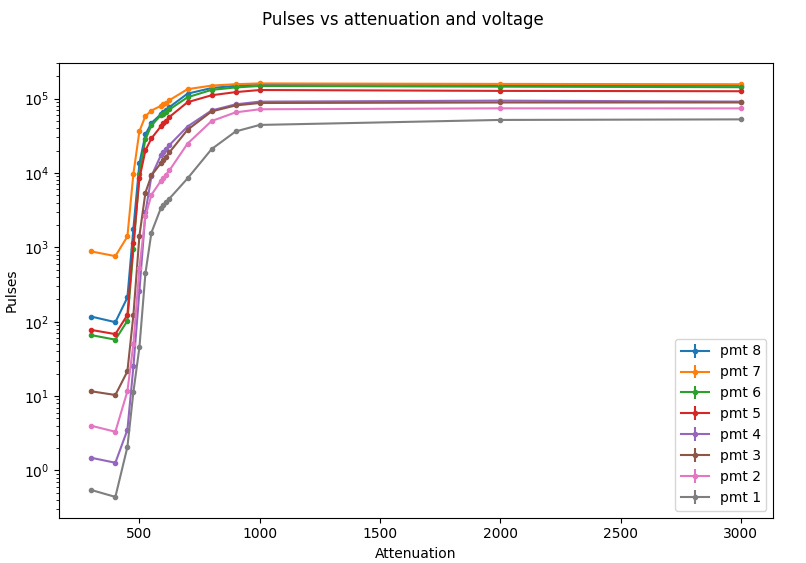
\includegraphics[width = 0.8\textwidth]{figures/Calibration.png}
\end{figure}

\end{frame}

\begin{frame}{Calibration of the pmt}

\begin{figure}[hbtp]
\centering
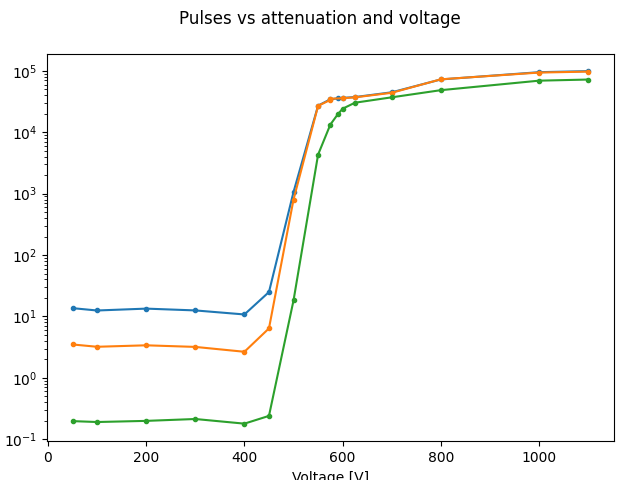
\includegraphics[width = 0.8\textwidth]{figures/CalibrationB.png}
\caption{Calibration of the pmt of detectorB, the threshold was selected at the edge of the knee for each pmt.}
\end{figure}

\end{frame}

\begin{frame}{Expected error}

The expected error is recostruncting the asymmetry is now computed:

\begin{gather*}
Var[A_{asym}] = Var[\dfrac{N_{\uparrow} - N_{\downarrow}}{ N_{\uparrow} + N_{\downarrow}}] \simeq \dfrac{Var[N_{\uparrow} - N_{\downarrow}]}{(N_{\uparrow} + N_{\downarrow})^{2}} \\
\frac{2Var[N]}{4N^{2}} = \frac{1}{2N} \qquad \sigma = \frac{1}{\sqrt{2N}}
\end{gather*}

This is the $\sigma$ supposing that the pmt's Counts are gaussian distributed, with $\mu$ equal to $\sigma^{2}$. The rms associated to the sample mean decrease as the $\sqrt{N_{measure}}$. 

Considering a $\mu = 10000$ and $3 \cdot 10^{6}$ data (often used during the simulation) the error is about $4 ppm$. Therefore, considering $5\cdot 10^{5}$ data, but $\mu = 40000$, a factor of $4$ more scattered electron (as we observed in the real data), we obtain an error of $\simeq 5ppm$.

\begin{figure}[hbtp]
\caption{Pmt 4, asymmetry on the left, pmt counts on the right}
\centering
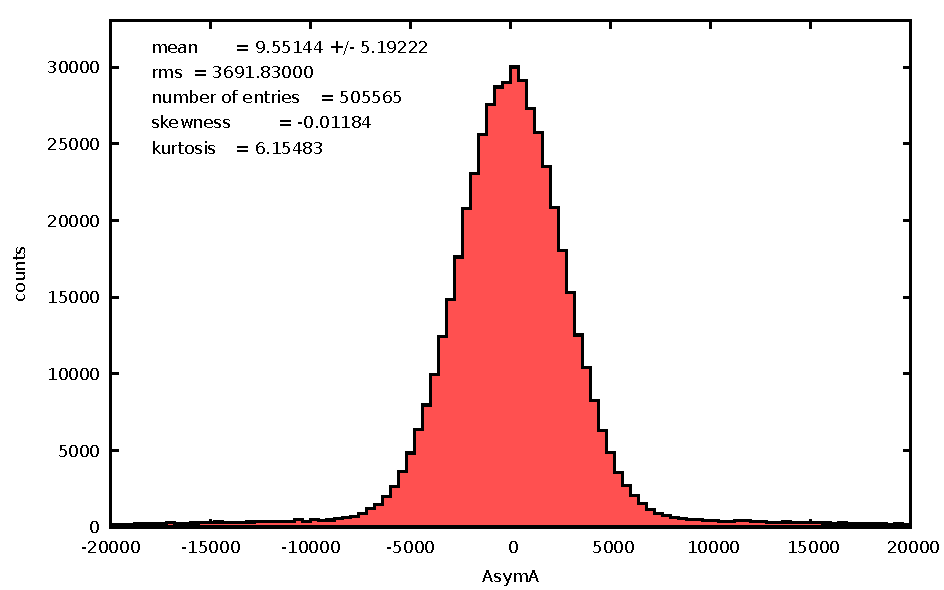
\includegraphics[width = 0.4\textwidth]{figures/ASYM_A4.pdf}
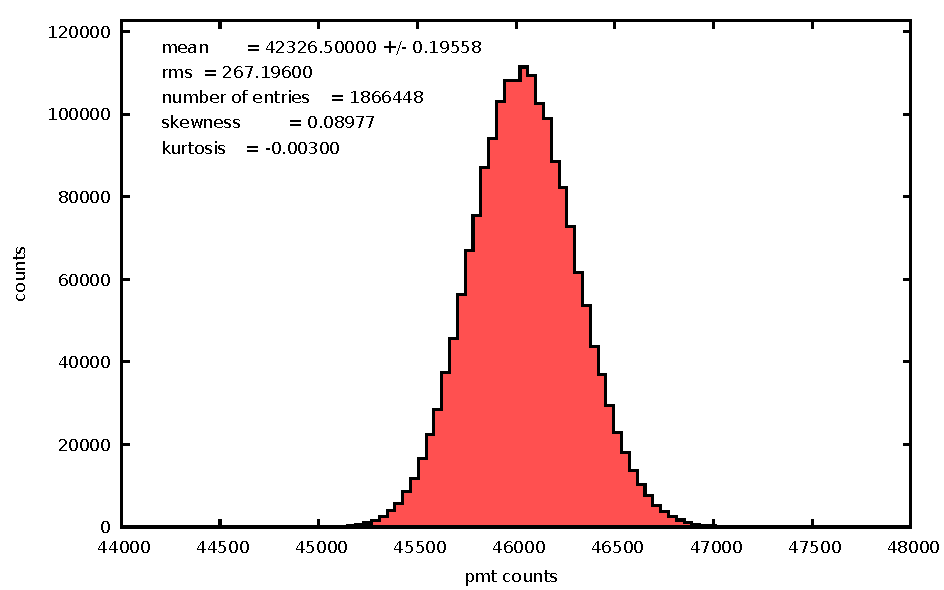
\includegraphics[width = 0.4\textwidth]{figures/pmtA4.pdf} 
\end{figure}

\end{frame}

\begin{frame}

Here a plot about the trend of the asymmetry as the data increases. The band is the error computed as showed in the previous slide, centered around the values of $+20ppm$

\begin{figure}[hbtp]
\centering
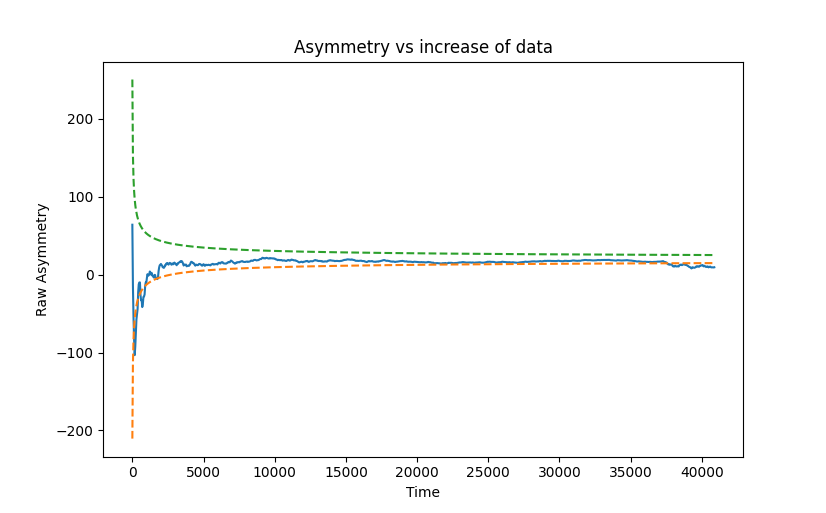
\includegraphics[width = 0.8\textwidth]{figures/Asymmetry_vs_data.png}
\caption{Raw asymmetry for pmt number 4 (as an example) as a function of the number of data}
\end{figure}

\end{frame}

\begin{frame}{Preliminary results}

For each pmt, we present the raw values of the asymmetry, obtained by subtracting the Raw current asymmetry, that is roughly $-1.11$ ppm , then we compute the averaged values:

\begin{figure}[hbtp]
\centering
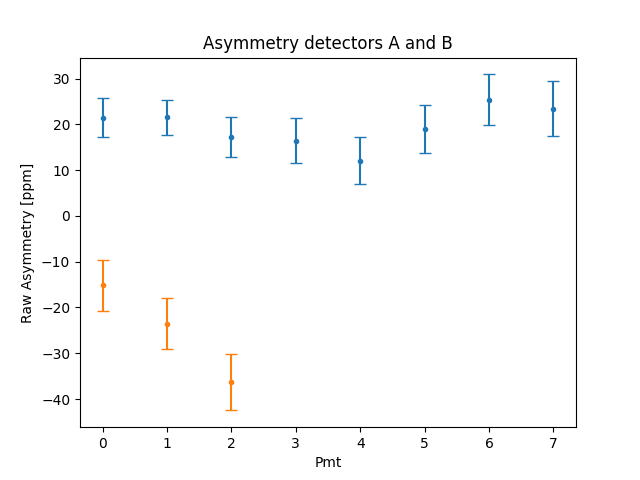
\includegraphics[width = 0.8\textwidth]{figures/RawResults.png}
\caption{•}
\end{figure}
\end{frame}

\begin{frame}{Preliminary results}
 
Combining the result of each pmt:

\begin{gather*}
\hat{Asym} =  \frac{\Sigma_{i} Asym_{i} \frac{1}{w_{i}}}{\frac{1}{w_{i}}} \qquad w_{i} = \frac{1}{\sigma^{2}_{i}}
\end{gather*}

We obtain the following:
\begin{equation}
A_{detA} = (20.45 \pm 1.6) ppm  \qquad A_{detB} = (-23.19  \pm 4.18)ppm
\end{equation}

\end{frame}
\end{document}